\documentclass[conference]{IEEEtran}
\IEEEoverridecommandlockouts
% The preceding line is only needed to identify funding in the first footnote. If that is unneeded, please comment it out.
\usepackage{cite}
\usepackage{amsmath,amssymb,amsfonts}
\usepackage{algorithmic}
\usepackage{graphicx}
\usepackage{textcomp}
\usepackage{xcolor}
\usepackage{hyperref}
\usepackage{marvosym}
\def\BibTeX{{\rm B\kern-.05em{\sc i\kern-.025em b}\kern-.08em
    T\kern-.1667em\lower.7ex\hbox{E}\kern-.125emX}}
\begin{document}

\title{Group17 Report: SVD-InST}

\author{\IEEEauthorblockN{Wu Shuwen}
\IEEEauthorblockA{
521030910087\\
\href{mailto:mike0510@sjtu.edu.cn}{mike0510@sjtu.edu.cn}
}
\and
\IEEEauthorblockN{Su Zhan}
\IEEEauthorblockA{
521030910112\\
\href{mailto:ililaoban@sjtu.edu.cn}{ililaoban@sjtu.edu.cn}
} 
\and
\IEEEauthorblockN{Yun Jiasheng}
\IEEEauthorblockA{
521030910093\\
\href{mailto:yjs180303@sjtu.edu.cn}{yjs180303@sjtu.edu.cn}
}
}

\maketitle

\begin{abstract}
We proposed our model SVD-InST combining SVD(Singular Vector Decomposition) and Stable-Diffusion to tackle Problem-4: Image-to-Image translation with generative model, in which we are required to translate realistic photo images into mural-style paints with provided datasets.
\end{abstract}

% \begin{IEEEkeywords}
% Style Transfer, Diffusion
% \end{IEEEkeywords}

\section{Introduction}
In this report, we performed SVD(Singular Vector Decomposition) on layers of the state of art pretrained model Stable-Diffusion on text-to-image generation as a finetuning technique. As Stable Diffusion is a text-to-image model, we utilize textual-inversion to align the desired style in our task with special symbols. Also, we'd like to call back about all our endeavors on proposing, implementing and perfecting our model.

\section{Related Works}
In this section of our report, we'd like to introduce part of the papers we've investigated and refered to during our project.

\subsection{Diffusion Models}
\subsubsection{DDPM}
DDPM\cite{ddpm} stands for Diffusion Models with Denoising Score Matching. It is a generative modeling framework that leverages diffusion processes and score matching for image synthesis. Diffusion models are a class of generative models that capture the underlying data distribution by iteratively transforming a simple initial distribution into the target distribution through a series of diffusion steps.

In DDPM, the diffusion process is combined with denoising score matching, which is a technique for estimating the score function of a probability distribution. The score function represents the gradient of the log-density function and provides valuable information about the data distribution. By estimating the score function, DDPM can learn to generate high-quality images with complex and diverse characteristics.

\subsubsection{Latent Diffusion Models} 
Latent Diffusion Models (LDMs)\cite{ldm} is a method for high-resolution image synthesis. LDMs decompose the image formation process into a sequential application of denoising autoencoders, allowing for state-of-the-art synthesis results. The authors propose training LDMs in the latent space of powerful pretrained autoencoders, which enables reaching a near-optimal point between complexity reduction and detail preservation. By introducing cross-attention layers into the model architecture, LDMs become powerful and flexible generators for various conditioning inputs such as text or bounding boxes.

\subsubsection{Stable-Diffusion}
Stable Diffusion is a deep learning, text-to-image model that was released in 2022. It is considered to be a part of the ongoing AI spring and is primarily used to generate detailed images conditioned on text descriptions. The model is based on diffusion techniques and is a latent diffusion model. Stable Diffusion is now one of the SOTA base models for text-to-image generation.

\subsection{Fine-tuning Techniques on Stable-Diffusion}

\subsubsection{DreamBooth}
DreamBooth is a technique that allows you to adjust the existing model weights of Stable Diffusion to generate a subject in different environments and styles. It involves providing a set of reference images of the subject, retraining the model to associate that subject with a specific word or embedding, and then prompting the new model using the special word. It was developed by researchers from Google Research and Boston University in 2022.

\subsubsection{Textual Inversion} 
Textual Inversion is a technique that works by figuring out the specific embedding that the model already associates with the reference images provided. It involves providing a set of reference images, determining the specific embedding associated with those images, and then prompting the new model using the embedding.

\subsubsection{Hyper-Networks}
Hyper-networks are widely used for fine-tuning pretrained models. On Stable Diffusion, hyper-networks are small neural networks that are attached to a Stable-Diffusion model to modify its style. They can be used in addition to checkpoint models to push the generated results towards a specific theme or aesthetic.

\subsubsection{LoRA}
LoRA (Local Randomized Adjustments) is another technique that can be used for fine-tuning Stable Diffusion. It involves adding microscopic new weights to the model instead of training an entirely new model. It allows for efficient fine-tuning of large-scale models like Stable Diffusion without the need to retrain the entire model. It was introduced by Microsoft researchers as a way to address the challenge of fine-tuning large-language models with billions of parameters, such as GPT-3, which can be computationally expensive and time-consuming.

\subsubsection{SVDiff}
Using SVD(Singular Value Decomposition) for Stable-Diffusion fine-tuning is first proposed in the paper titled "SVDiff: Compact Parameter Space for Diffusion Fine-Tuning" in 2023.\cite{svd} Before that, SVD
has also been used for fine-tuning other large pretrained models such as Segment Anything Model(SAM).

The authors propose fine-tuning the singular values of the weight matrices to create a compact and efficient parameter space. This approach reduces the risk of overfitting and language drifting.The proposed SVDiff method has a significantly smaller model size compared to existing methods, making it more practical for real-world applications.

It is worth emphasizing that before SVDiff is proposed, LoRA used to be smallest model for Stable-Diffsuion fine-tuning. Compared to LoRA, SVDiff has approximately 0.6 million fewer trainable parameters. In the respect of storage and inference, the file size of SVDiff is less than 1MB, while the size of a LoRA file ranges from about 30 to 150 MB according to the number of the networks injected. More specifically, with rank one, the storage and update requirements for the W matrix of shape M × N in SVDiff are min(M, N) floats, compared to (M + N) floats
for LoRA.

\subsection{Style Transfer}
Style-Transfer for artistic images has become a quite mature field in recent years. Many models and methods have been proposed. 

\subsubsection{GAN Models for Style Transfer} 
GAN models prove to be strong in generating tasks, including Style-Transfer.Multiple Style-Transfer models based on GAN(Generative Adverserial Networks) have been proposed in the past few years. 

\textbf{CycleGAN}\cite{cycle}, introduced by Zhu et al. in 2017, is designed for unpaired image-to-image translation. It aims to learn mapping functions between two domains without requiring paired training data. CycleGAN utilizes a cycle consistency loss to enforce the translated images to be able to reconstruct the original images when translated back to the original domain.

\textbf{StarGAN}\cite{star}, proposed by Choi et al. in 2018, is a GAN-based model that enables multi-domain style transfer. Unlike CycleGAN, StarGAN can handle multiple domains with a single model. It introduces a novel concept of a "domain label" that allows the model to control the style transfer between different domains using a single generator and discriminator network.

\textbf{BalaGAN}\cite{bala}, presented by Berthelot et al. in 2019, is a GAN model specifically designed for attribute manipulation in facial images. It focuses on preserving the identity information while modifying specific attributes of the input image. BalaGAN employs a novel adversarial loss and a feature matching loss to guide the generator in producing realistic and attribute-modified images.


\subsubsection{Transformer Based Style Transfer}
Transformer-based models have recently reached SOTA in multiple fields. For Style Transfer, there're also transformer based models that show great performance.S

\textbf{StyTr$^2$}\cite{stytr} is a transformer-based approach for image style transfer. Traditional neural style transfer methods often struggle with biased content representation due to the locality in convolutional neural networks (CNNs). To address this issue, StyTr$^2$ takes long-range dependencies of input images into account. It consists of two different transformer encoders, one for generating domain-specific sequences for content and another for style. These encoders are followed by a multi-layer transformer decoder that stylizes the content sequence according to the style sequence. The paper also proposes a content-aware positional encoding (CAPE) method, which is scale-invariant and more suitable for image style transfer tasks. 

\subsubsection{Latent Diffusion Models for Style Transfer} 
Style-Transfer models based on Latent Diffusion Models have been emerging since the model Stable-Diffusion made a hit. The perfect performance of Latent Diffusion Models have changed every thing in AIGC and Style-Transfer is not an exception.

\textbf{InST}\cite{inst}, or "Inversion-Based Style Transfer with Diffusion Models", introduced an inversion-based approach that learns the key information of an image and uses it to guide the synthesis process. They leverage diffusion models and inversion techniques to achieve this. The method involves obtaining the textual description of the image style, which is considered as "new words" that do not exist in normal language. The inversion module learns key features from an image and generates the corresponding textual embedding. The diffusion models conditioned on the textual embedding can then produce new images with the learned style of the reference painting.

\textbf{ArtFusion}\cite{artfusion} utilizes innovative Dual Conditional Latent Diffusion Probabilistic Models (Dual-cLDM) to enhance the style transfer process. Dual-cLDM combines a Variational Autoencoder (VAE) and a diffusion backbone. The VAE reduces the spatial dimensionality of the image while preserving its semantic essence, resulting in a concise, low-dimensional latent space. The diffusion backbone operates within this latent space, eliminating the need to handle redundant data in the high-dimensional pixel space, thus reducing computational burden.

\begin{figure}[!t]
\centering
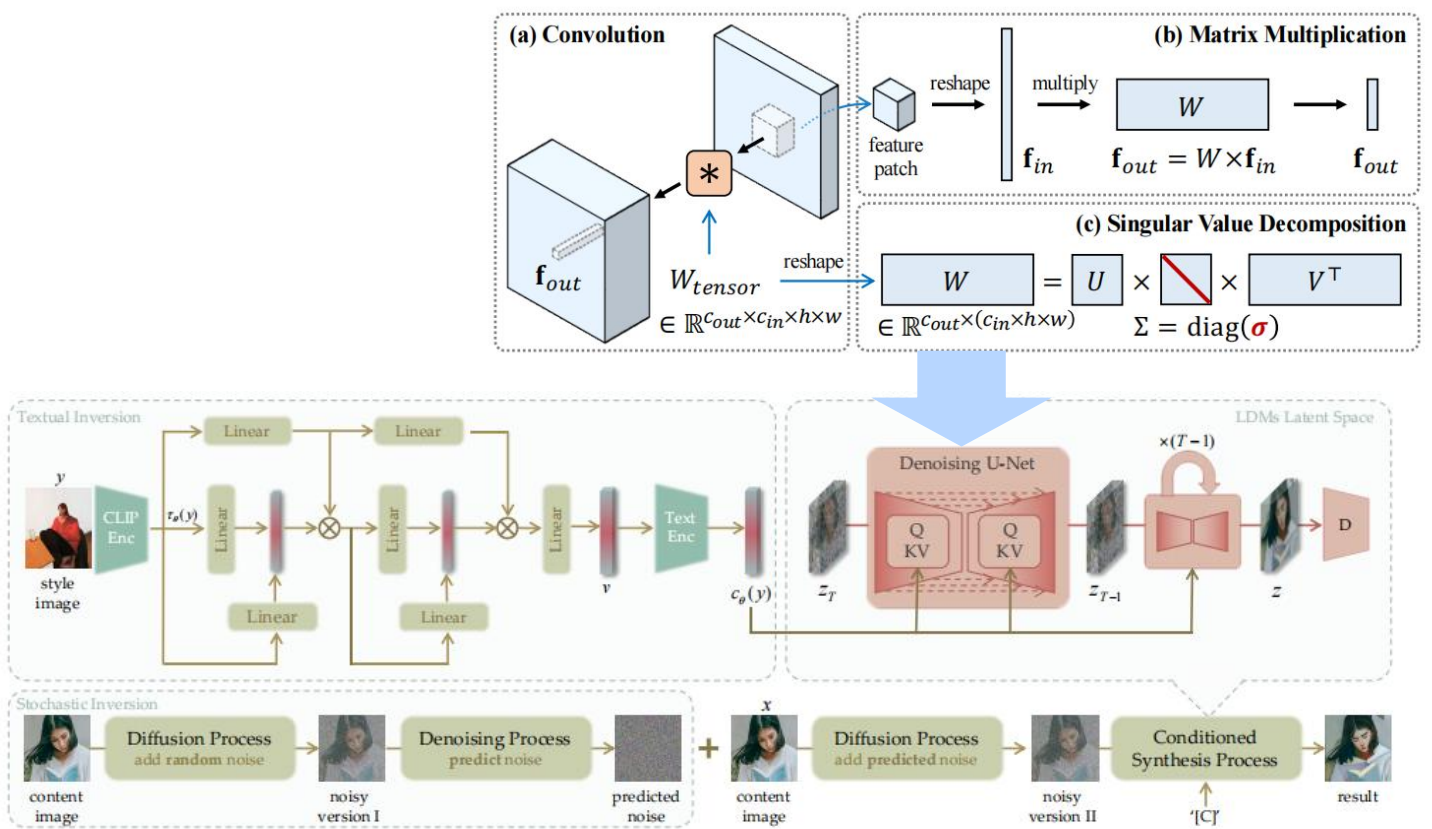
\includegraphics[width=3.5in]{SVD-InST.png}
\caption{Overview of architecture of SVD-InST. 
Both textual inversion and SVDiff are utilized in our model. Textual inversion aligns the special symbols and the desired style. SVDiff fine-tunes the latent diffusion model to improve its performance on one specific task.}
\label{approach_svd}
\end{figure}

% \newpage
\section{Methods}

\subsection{Overview}


In this work, we use textual inversion as the basis of our framework for Style Transfer. Special symbols and our desired style are aligned to each other through a CLIP text embedding we train.

Also, to enhance the Stable Diffusion Model's performance on our single Style Transfer task, we fine-tune the pretrained latent diffusion model weights to make it perform better for this one specific task, without considering its performance on generalized image generation. Specifically, we perform SVD on layers of the latent diffusion model and update the singular values, like what SVDiff does.

\subsection{Textual Inversion}

Stable Diffusion Models utilize CLIP text embedding as the condition in text-to-image generation. 

The CLIP text encoding contains two processes of tokenization and parameterization. An input text is first transformed into a token, which is an index in a pre-defined dictionary, for each word or sub-word. After that, each token is associated with a distinct embedding vector that can be located using an index. 

We set the concept of a picture as a placeholder “[C]”,  and its tokenized corresponding text embedding as a learnable vector $\hat{v}$. 
[C] is in the normal language domain, and $\hat{v}$ is in the textual space. 

By assuming a [C] that does not exist in real language, that is, special symbols in our implementation, we create a “new word” for the Nine Color Mural artistic style. 

We embrace the learning method based on multi-layer cross attention proposed by the author of InST.  The input artistic image is first sent into the CLIP image encoder and gives image embeddings. By performing multi-layer attention on these image embeddings, the key information of the image can be quickly obtained. The CLIP image encoder $\tau_\theta$  projects y to an image embedding $\tau_\theta(y)$. The multi-layer
cross attention starts with $v0 = \tau_\theta(y)$. Then each layer is
implementing $Attention(Q, K, V ) = softmax(\frac{QK^T}{\sqrt{d}})$
with:
$$
Q_i = W^{(i)}Q \cdot vi ,
K = W^{(i)}K \cdot τθ(y),  
V = W^{(i)}V \cdot τθ(y)
$$
$$
v_{i+1} = Attention(Q_i, K, V )
$$
% During training, the model is conditioned by the corresponding text embedding only. To avoid overfitting, we apply a dropout strategy in each cross-attention layer which
% set to 0.05.



\subsection{SVD(Singular Vector Decomposition)}

\begin{figure}[!t]
\centering
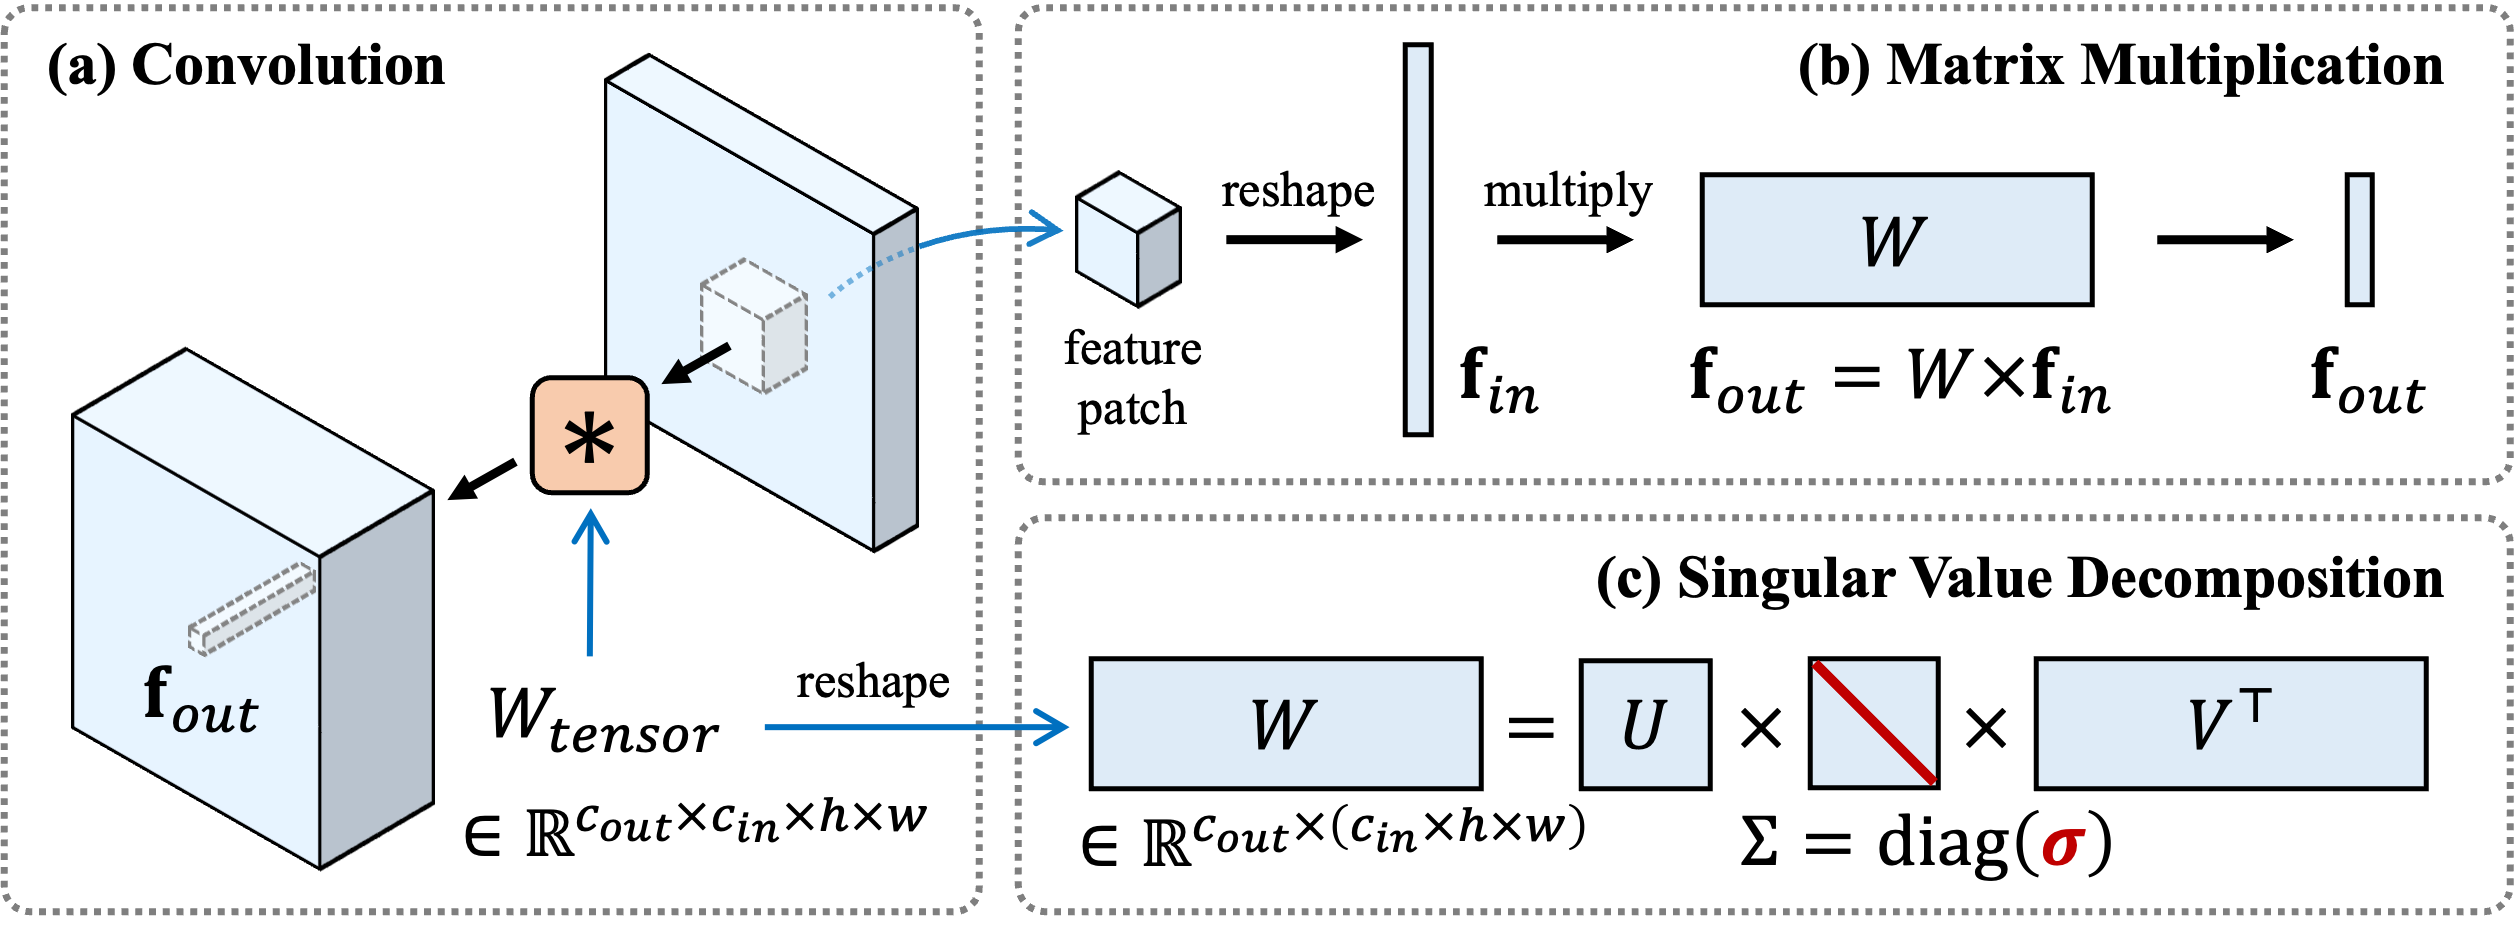
\includegraphics[width=2.5in]{approach_svd.png}
\caption{Performing singular value decomposition (SVD) on
weight matrices. In an intermediate layer of the model, (a) the
convolutional weights Wtensor (b) serve as an associative memory. (c) SVD is performed on the reshaped 2-D matrix W}
\label{approach_svd}
\end{figure}
As is shown in Fig.2, for a layer in the model to be fine-tuned, its original weight matrix is denoted as W, Then, its SVD equation can be expressed as $W = U\Sigma{}V^T  $, where $ \Sigma = diag(\boldsymbol{\sigma})$ and $ \boldsymbol{\sigma} = [\sigma_{1} , \sigma_{2},...]$. 

In our implementation, the SVD is a one-time computationm, performed before the first iteration in the training process, and can be cached. For each decomposed layer W, once the SVD algorithm is performed, only the diagonal matrix $\Sigma = diag(\boldsymbol{\sigma})$ will be marked as trainable. $U$ and $V^{T}$ are frozen in the training process. 

The updated weight matrix can be re-assembled by:
$$ W_{\delta } = U \Sigma _{\delta } V^\top ~~ \text {with} ~~ \Sigma _{\delta }=\text {diag}(\text {ReLU}(\sigma +\delta )) $$


\subsection{Optimization Scheme}

For the CLIP embedding, the optimization goal can be defined as:
$$\hat{v} = argmin_v
E_{z,x,y,t} [\|\epsilon {-} \epsilon_\theta (z_t, t, MultiAtt(\tau\theta(y))\|^2_2
]$$
where $z \sim E(x),\epsilon \sim N (0, 1). \tau_\theta$ and $\epsilon_\theta $are fixed during
training. In this way, $\hat{v}$ can be optimized to the target area efficiently.


For the singular values diagonal matrix $\Sigma$, the loss function can be expressed as:
$$ \mathcal {L}(\delta ) &= E_{z ^*,c ^*,\epsilon ,t}{\|\hat {\epsilon }_{\theta _\delta }(z _t^* | \bc ^*) - \epsilon \|^2_2}$$
% +\lambda \mathcal {L}_{pr}(\delta )$$
% with$$ \nonumber \\ \mathcal {L}_{pr}(\delta ) &= E_ {z ^{pr},c ^{pr},\epsilon ,t}{\|\hat {\epsilon }_{\theta _\delta }(z _t^{pr} | c ^{pr}) - \epsilon \|^2_2}$$

\section{Experiments&Results}
We conducted our experiments on multiple models, including GAN-based, transformer-based, and diffusion models. For each model we trained, we kept the training settings provided by the authors so that the comparison would be relatively fair. The results of tested models and our SVD-InST model are shown in FIg.3.

\begin{figure}[!t]
\centering
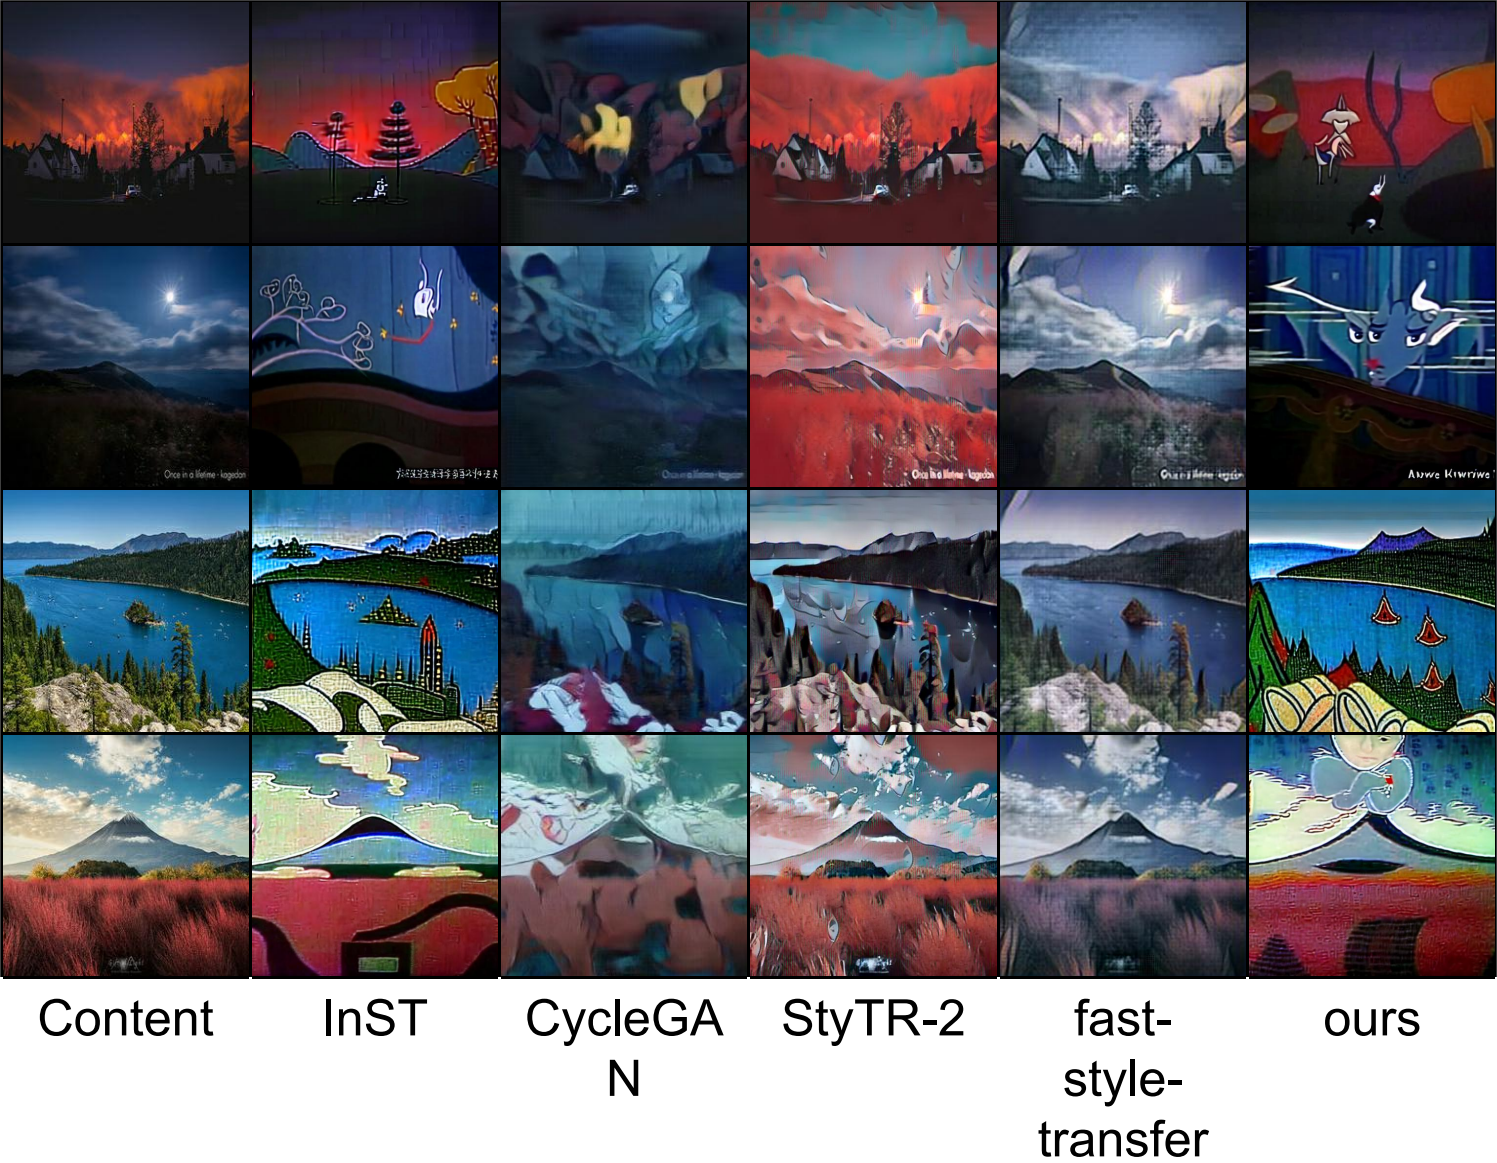
\includegraphics[width=3.5in]{result1.png}
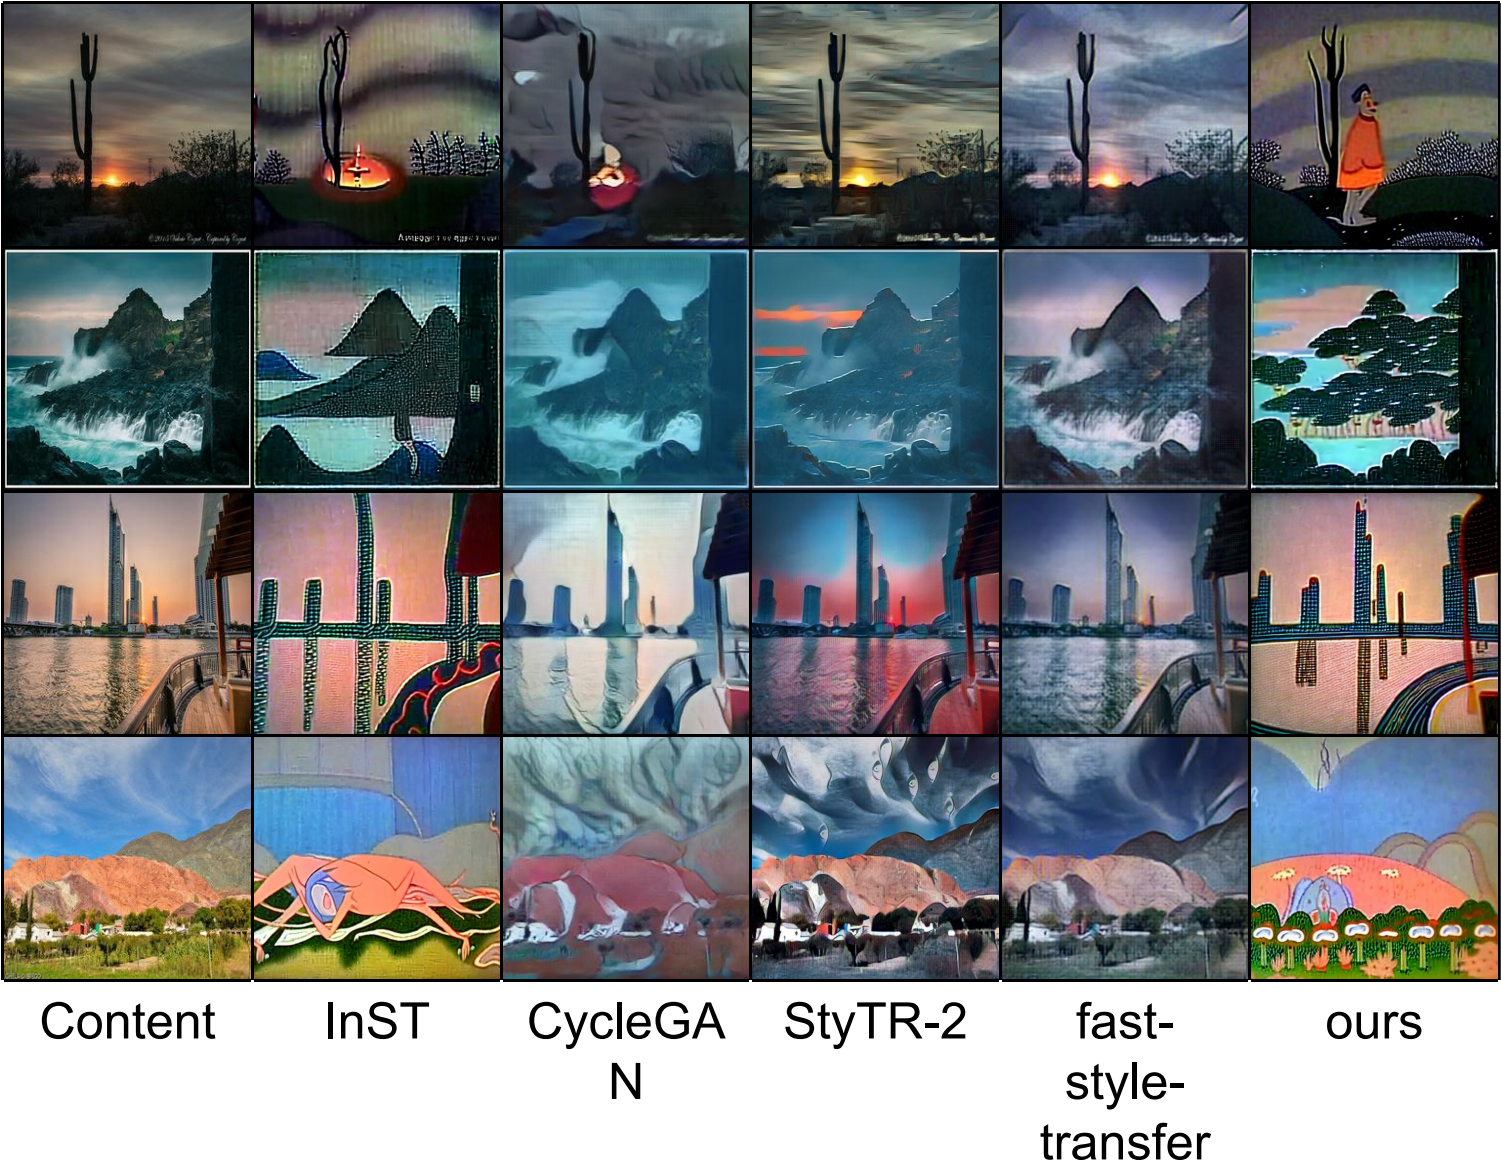
\includegraphics[width=3.5in]{result2.png}
\caption{Results of different models compared to ours. Strength of InST and our model are set to 0.8.}
\label{approach_svd}
\end{figure}


\subsection{SVD-InST}



\subsubsection{Implementation}
We implemented an SVD-Unet Module adapted from OpenAI's implementation for Unet-Model. The SVD-Unet is then used as the diffusion model of the Stable Diffusion Model architecture. By first implementing basic SVD layers, we were able to easily translate any pytorch module into one similar module with SVD option.

In our model, UNet architecture is used as a generator within the latent diffusion framework. Instead of directly sampling from the noise distribution, the generator network takes the diffused latent variables as input and produces an image. This allows the generator to leverage the learned hierarchical representations of the UNet architecture to generate high-quality images with coherent and meaningful structures.

\subsubsection{Training}
Stable Diffusion Models utilize CLIP text embedding as the condition in text-to-image generation. Before we start training, We first load the pretrained weights from SD1.4 for the LDM part and the default pretrained weights provided by CLIP. Then, we fine-tune the embedding of CLIP and Singular Values of SDM in our training process.

The base learning rate was set to 0.001. The synthesis process takes the same time as SDM, which depends on the steps. 

As soon as the training process is finished, the CLIP embedding weights are first saved as an embedding file. Then the spectral shifts $\delta$ on singular values of the latent diffusion model are selected from its state dictionary and are saved to another file.
\subsubsection{Inference and Tests}
To initiate our SVD-InST for inference process, we first load the original SD1.4 checkpoint and the train embedding. Then we perform SVD on each module of the diffusion model. Finally, the spectral shifts are loaded to the modify the diffusion model.

After initiation, SVD-InST is ready for inference. We generated 10 images for each content image from the test photo directory with different seeds and strength set to 0.8. We then tested LPIPS and FID performances with these images.

\subsection{InST}
We test vanilla InST using the training settings provided by the author for single&few image style transfer.

Just the same as what we did testing SVD-InST, we also generated 10 images for each content image from the test photo directory with different seeds and strength set to 0.8. LPIPS and FID performances are also tested with these images.

\subsection{GAN models}
For GAN models, we tested CycleGAN, StarGAN, and BalaGAN. We first devided the training data as GAN models require: Both content images(photos) and style images(Nine Colored Mural pictures) are divided into a training part and a test part, which is totally four directories of images. For the training process of generators and discriminators, the training part of content images and style images are loaded and used. During the loss calculation part of the recursive training process, the test images are used.

\textbf{BalaGAN} In our experiment, we found that actually, BalaGAN is not so suitable for our style transfer task, as it focuses on preserving the identity information while modifying specific attributes of the input image instead of pure artistic styles.

\textbf{CycleGAN and StarGAN} CycleGAN and StarGAN both show fine performance in general style transfer task. CycleGAN is good at unsupervised domain adaptation, allowing the conversion of images from one domain to another without paired training data. StarGAN, on the other hand, focuses on multi-domain image translation, allowing the simultaneous handling of multiple different domains within a single model. 

In our experiments, StarGAN prove to be not as robust as CycleGAN. Training StarGAN on such datasets results in over-fitting quite easily. On the other hand, CycleGAN perfectly transfer the test photos into the desired style.

We tested FID of images generated by CycleGAN but not LPIPS, as CycleGAN is not capable of generating diversified images with a same setting.

\subsection{Transformer-based Models}
For this part, we tested StyTR$^2$ and fast-style-transfer. 

\textbf{StyTR$^2$} According to the author's guidance, we loaded pretrained VGG encoder weights for StyTR$^2$, froze it and trained only the decoder. After that, we generated the outcome images look quite good. Also, we tested FID of imaged generated by StyTR$^2$.

\textbf{Model Simplification} Besides, we also tried to simplify the model architecture of StyTR$^2$, by reducing the number of pooling and up-sampling layers. But such a simplified model turned out to be not robust and had worse performance than the full-size model. Also, reducing the depth of VGG encoders and decoders reduces the model's capability of extracting characters from different scales.

\textbf{Fast-Style-Transfer} Continuing with the fast-style-transfer portion, fast-style-transfer operates by applying a pre-trained model to quickly transform images into a desired style. The model architecture is based on a pre-trained neural network, specifically using the VGG19 architecture. And the pre-trained model is fine-tuned using the content images.Throughout the training process, the model learns to minimize the difference between its stylized outputs and the style of the chosen style image. Checkpoints of the trained model are then saved for subsequent evaluation. In the evaluation phase, these checkpoints are utilized by the model to generate style transfer images.



\section{Analysis}



\begin{table}[h!]
  \begin{center}
    \caption{Training Results}
    \begin{tabular}{l|c|r|l|c} % <-- Alignments: 1st column left, 2nd middle and 3rd right, with vertical lines in between
      \textbf{Model} & \textbf{FID} & \textbf{LPIPS}\\
      \hline
      InST &127.5& 0.53\\
CycleGAN& 178.3 &/\\
StyTR-2 &171.3& /\\
fast-style-transfer&172.7 &/\\
ours &125.1 &0.54
    \end{tabular}
  \end{center}
\end{table}
Examples of generated images are shown in Fig.3.

The FID and LPIPS scores of our model compared to diifferent models are as shown in TABLE 1. The number of parameters of the whole SVD-InST is 1.5B, while the trainable parameters count to 3.7M. It is obvious that the frozen SD1.4 takes up most of the parameters in the whole model.


\begin{thebibliography}{00}
\bibitem{ddpm}Denoising Diffusion Probabilistic Models
\bibitem{ldm}High-Resolution Image Synthesis with Latent Diffusion Models
\bibitem{cycle}Unpaired Image-to-Image Translation using Cycle-Consistent Adversarial Networks
\bibitem{star}StarGAN: Unified Generative Adversarial Networks for Multi-Domain Image-to-Image Translation
\bibitem{bala}BalaGAN: Image Translation Between Imbalanced Domains via Cross-Modal Transfer
\bibitem{inst}Inversion-Based Style Transfer with Diffusion Models
\bibitem{artfusion}ArtFusion: Controllable Arbitrary Style Transfer using Dual Conditional Latent Diffusion Models
\bibitem{svd}SVDiff: Compact Parameter Space for Diffusion Fine-Tuning
\bibitem{stytr}StyTr2: Image Style Transfer with Transformers
\end{thebibliography}


\end{document}
